\chapter{Discussion}
\label{section:discussion}
%The goal of this thesis is build a scalable approach for MILP trajectory planning. The target vehicles are multirotor UAVs, so the results in the previous section need to be analyzed in that context. \\
%The first step is analyzing whether or not the approach is actually scalable enough when planning the trajectory for this kind of vehicle through complex environments.\\
%Afterwards, the other experiments demonstrate the importance of some of the parameters used in the algorithm. The results provide insight in the limitations of the current approach, and how it may be improved in the future.
%\par
The main focus points during this these were the performance and stability of the algorithm. Most decision were made with either performance or stability in mind, and often both. TODO: preview with refs
\section{Performance}
On the performance side, it is clear that the new algorithm with preprocessing is much faster than solve the pure MILP problem without preprocessing. Comparing the new algorithm to the pure approach is very difficult since the challenging scenarios for the new algorithm simply cannot be solved with the pure approach.
\par
When it comes to scalability, there are few noteworthy observations to make. 
\subsection{Path Length Scalability}
The first is that the time needed to solve each MILP subproblem does not depend on the length of the trajectory or the size of the world. Accounting for variations due to obstacle density, the average MILP solve time for scenarios using the same dataset (San Francisco or Leuven) are very similar. Since the amount of segments scales linearly with the path length, the MILP part of the algorithm also scales linearly with the length of the initial path. This is in stark contrast with the exponential worst-case performance of the pure MILP approach\\
However, this exponential complexity has not been eliminated. It has been shifted to the initial path planning algorithm, Theta*. This algorithm still has exponential worst-case complexity with respect to the length of the path. While Theta* does limit the scalability regarding the size of the world, it is a much easier problem to solve. It is part of the A* family of path planning algorithms which have been the subject of a large body of research.
\par
The algorithm separates the "routing" aspect from the trajectory planning aspect of the problem. The exact properties of the initial path are not very important. What matters is that it determines where and when to turn. By the time the MILP solver runs, the navigation aspect of the problem has already been solved. The MILP solver only needs to find a viable trajectory. The two aspects of the problem are solved separately, making both of them easier to tackle.
\par
I believe that identifying that these two aspects can be solved separately is the key insight that made the performance improvements possible. Solving these aspects separately means that the optimal trajectory is unlikely to be found. However, at this point that seems like a necessary sacrifice for long term trajectory planning through complex environments. I am not aware of any algorithm that scales as well as my algorithm does, and also finds the optimal trajectory.

\subsection{Obstacle Density Scalability}
The second observation is that the density of the obstacles plays a large role in the scalability of the algorithm. The San Francisco and Leuven scenarios are very similar, except for their obstacle density. The Leuven scenario has a significantly higher density of obstacles and is also much harder to solve. Without preprocessing, the scalability of the MILP problem is limited by the total amount of obstacles. Because each MILP subproblem in my algorithm is roughly the same size, the total amount of obstacles is no longer the limiting factor. The density of the obstacles is the limiting factor in my algorithm.
\par
The Leuven scenarios can still be solved in an acceptable amount of time, but I do not believe that this will be the case if the density is increased even more. Luckily, the Leuven dataset is more detailed than it needs to be. Each building in the city is represented separately, even when multiple buildings are connected. It should be possible to reduce the obstacle density substantially with a minimal amount of effort. Figure \ref{fig:leuven-dense} shows a dense region in the Leuven dataset where there is a lot of room for improvement.

\begin{figure}[h]
	\centering
	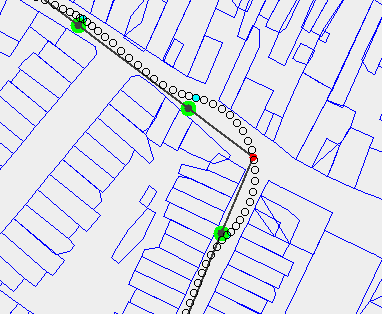
\includegraphics[width=0.5\textwidth]{leuven-dense}
	\caption{One of the denser regions in the Leuven dataset}
	\label{fig:leuven-dense}
\end{figure}

Given that the Leuven dataset is so unoptimized for this purpose and the algorithm still completes on average on the order of seconds per segment, I believe that the scalability with regards to the obstacle density is acceptable.

\subsection{UAV Agility} 
The last observation is the importance of the agility of the UAV. The algorithm was developed with high-end consumer to professional grade multirotor UAVs in mind. These are very agile vehicles capable of impressive feats of acrobatics when properly piloted. This agility is one of the assumptions this algorithm is based on. The UAV must be able to hover and accelerate quickly.
\par
The results from the UAV agility experiment in section \ref{subsec:agility} show that these assumptions are indeed a critical part of the performance of the algorithm. The algorithm fails when faced with UAVs with an (unreasonably) low agility. 
\par
This reliance on agility is one of the factors that made the dramatic improvement in performance possible, but it also limits the applicability of the algorithm. However, the goal of this thesis was not to developed a general algorithm. The algorithm performs well for reasonable estimates of the agility of a multirotor UAV. On top of that, the agility of any UAV can be increased by limiting its maximum velocity\footnote{Limiting the maximum velocity of UAVs with a low acceleration when navigating through a city seems like a wise decision anyway. Such a UAV would not be able to react to unexpected obstacles quickly, so having it fly at a high velocity through the city seems like a dangerous proposition.}.


\section{Stability}
For the algorithm to be useful, it must be stable. The first aspect of stability is whether or not it can find a solution. If the algorithm is capable of finding a solution, it should find that solution every time. It should also be able to solve problems with a similar difficulty as well. The second aspect is that the solution for the same problem should always be similar. There should be no large differences in the trajectory scores when the same problem is solved multiple times, nor should there be a large difference between very similar problems. This is also applies to the execution time. The execution time for similar problems should also be similar without large variations.
\par
My algorithm can find a solution most of the time. Due to what I believe to be a bug, it occasionally fails to find a solution. I was not able to fully understand why the bug occurs, but I believe it can probably be fixed.  
\par
The stability of the trajectory scores are excellent. All trajectories found are scored within a few percentage points of each other. When it comes to the execution time, there is more variation. However, with a standard deviation is around 10-15 \% of the mean execution time, I believe that the stability is still acceptable for offline trajectory planning.
%The general performance results show that the algorithm is capable of planning a long trajectory through complex environments. Even for the smallest scenario, the solver struggles to find a trajectory for a pure MILP problem without preprocessing. With my algorithm, the UAV can successfully navigate an entire city. \\
%
%The stability experiment shows that, for the most part, my segmentation approach preserves stability. There are occasional failures which seem to be caused by a bug. However, assuming this bug can be fixed the stability of the algorithm 
%
% Overall I am not entirely satisfied with the stability of my current implementation, however I do believe the small issues around segment transitions can be resolved. \\\\
%
%The results show a large improvement in scalability in certain realistic scenarios, but the choice of those scenarios has drastically impacted the algorithm I have developed.\\
%
%During development, I have always used realistic approximations of the capabilities of multirotor UAVs. Those can reach high accelerations but have relatively low maximum velocities compared to what fixed-wing aircraft can achieve. This makes those vehicles very agile, which is one of the contributing factors to their recent popularity. \\
%The assumption of this agility means that my algorithm cannot be applied to UAVs which do not have that property. One of the properties my algorithm uses often is the maximum acceleration distance, which is the distance in which the UAV can always come to a complete stop. This works fine with multirotor UAVs, but is a meaningless concept when dealing with fixed-wing UAVs which cannot stop at all during flight. \\
%However, those kinds of low-agility UAVs are unlikely to be deployed at low altitudes in dense city centers exactly because they lack agility. Even with perfect planning, cities are very unpredictable places. An multirotor UAV is much more likely to be able to safely react to an unexpected obstacle than a fixed-wing UAV. \\
%While I picked out fixed-wing UAVs as an example, the same arguments hold for any kind of UAV that either cannot hover or has low agility. Some UAVs may be able to hover, but are not very agile due to a high maximum velocity and low acceleration. In this case, the agility can be improved by reducing the maximum velocity.\\ \\
%
%The density of obstacles is also an extremely important factor. The Leuven scenario is significantly harder than the San Francisco scenario because the obstacles are smaller and closer together. Not only are the obstacles closer together, but they are also polygons and can have many more edges per obstacle. For scenarios where the obstacles are significantly denser or complex than in the Leuven scenario, the approach may not improve the performance enough. \\
%On the other hand, the Leuven map is much more detailed than is required for navigation. Many obstacles could be merged together without a significant on possible trajectories. The obstacles could also be simplified, reducing the amount of edges per obstacle. Given that the Leuven map is unprocessed except for calculating the convex hull of each obstacle, the algorithm should be able to handle most real world maps when properly prepared.
%
%Given these considerations, I conclude that my approach meets the basic requirements. The assumptions behind the design of the algorithm seem to be valid based on experiments.

\section{Important parameters}
\label{section:imp-params}
During development of the algorithm I settled on sensible default parameters which balance both the performance of the algorithm and the quality of the resulting trajectory. The experiments which tested different values for those parameters provide a deeper insight in the effects of those parameters. Many of those insights point to possible improvements to the current algorithm.

\subsection{Time Step Size and Maximum Time}
From the time step size experiment (section \ref{subsec:timestep}) and maximum time experiment (section \ref{subsec:maxtime}) it becomes clear that the amount of time steps in each segment has a very large effect on the performance of the algorithm. The time step size should be chosen so the quality of the trajectory is high enough to be usable, without being more detailed than necessary. How large the time step size should be will depend on the specific use case. The maximum time should always be as low as possible, while still ensuring that the goal can be reached in that time. \\
By combining the effects of those parameters, the algorithm could be made faster without suffering a quality penalty. For each  segment, the algorithm could first solve a MILP problem with a conservative maximum time and a large time step size. The solution to this problem shows how much time the UAV needed to reach its goal in that segment. This value can be used as a much tighter maximum time in a MILP problem with a smaller time step size. While I did not have time to properly implement this, a quick-and-dirty test showed promising results.  Using this method and solving the segments first with a time step size of $0.5s$, the San Francisco scenario MILP solve time dropped from 32s to 10s. For the Leuven scenario the MILP solve time dropped from  136s down to 38s. In both cases, the execution time was cut by more than two thirds without impacting the quality of the trajectory.

\subsection{Approach Margin}
The approach margin experiment (section \ref{subsec:approach-margin}) shows that having some approach margin is beneficial, but that the gains are often relatively small. Overlapping the segments by just 5 time steps already results in a significantly better trajectory than a very large approach margin. Because of this, I believe that my idea that a larger approach margin leads to more efficient approach is not accurate. I suspect that the slight improvements in trajectory score when increasing the approach margin are caused by simply having fewer segments. Or to put it more accurately: it is caused by having fewer transitions between segments. Overlapping the segments smooths out bad transitions between those segments. A larger approach margin does not improve bad transitions, it only guarantees that the UAV can correct for it in time. These bad transitions are not immediately obvious when the UAV is constantly maneuvering, but they become very clear when the UAV is flying straight. Figure \ref{fig:sf-wavy2} shows a case where the UAV is not moving entirely along the path after a turn. This is corrected, but it starts an oscillation along the trajectory that takes many segments to die down. In Figure \ref{fig:sf-wavy2b}, the slight overlap of the segments prevents that oscillation from starting in the first place. 
\begin{figure}[h]
	\centering
	
	\begin{subfigure}[t]{.4\textwidth}
        		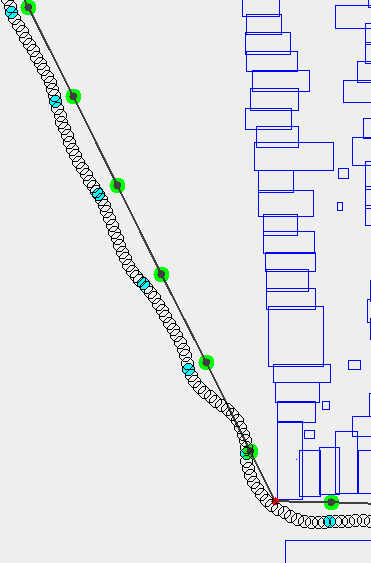
\includegraphics[width=\textwidth]{img/sf-wavy2}
        		\caption{}
        		\label{fig:sf-wavy2}
	\end{subfigure}
	\hfill
	\begin{subfigure}[t]{.4\textwidth}
        		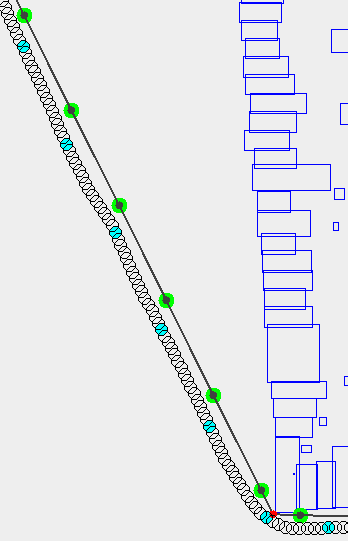
\includegraphics[width=\textwidth]{img/sf-wavy2b}
        		\caption{}
        		\label{fig:sf-wavy2b}
	\end{subfigure}	
	
        
    \caption[The effect of overlapping obstacles on oscillations in the trajectory]{Without overlapping the segments, oscillations tend to occur in the trajectory as seen in \ref{fig:sf-wavy2}. Even a small amount of overlap is an effective countermeasure as seen in \ref{fig:sf-wavy2b}.}
    \label{fig:sf-wavy}
\end{figure}
With my current algorithm there is a high performance cost involved with overlapping the segments. However, I do not believe this necessarily has to be the case. This is definitely something to look at in future work.

\section{Genetic Algorithm}
The genetic algorithm is the part of the thesis that got the least attention. This is mainly because the genetic algorithm itself is not an essential part of the trajectory planning algorithm. It is used to grow the convex safe region, and the current genetic algorithm does that well enough. Due to time constraints I have omitted detailed parameter tuning of this genetic algorithm.
\par
Either way, the genetic algorithm is very crude. A genetic algorithm was chosen to grow the convex safe region because it is a quick way to get a reasonably good result.  Since it never was the most pressing issue in the project, it never got replaced by a more refined algorithm (genetic or otherwise). 

\section{Future work}
\label{section:future}
There are several extensions and improvements which may improve the performance of the algorithm or the quality of the trajectory. These extensions may also improve the general utility of the algorithm, making it useful for more different use cases

\begin{itemize}
\item As discussed in section \ref{section:imp-params}, solving each segment multiple times with different parameters can result in performance improvements. However, when combined with the observation that the segment transition can be improved with overlapping segments, I believe that a more drastic change may be in order. Solving the segments first with a high time step size may also be used in combination with a high amount of overlap with other segments. This rough trajectory does not only contain information on the time needed to solve a segment, but may also be used to subdivide the segments even further.
\item Another step is extending this approach to 3D. The extra degree of freedom will likely come at a significant performance penalty, so this was not attempted during the thesis. One of the likely difficulties with the preprocessing as presented is that it treats all dimensions the same. This is fine for the horizontal dimensions, but due to gravity, movements the vertical dimension have different characteristics. The maximum acceleration of the UAV can no longer be assumed to be the same in all directions.\\
A possible mitigation to the increasing complexity of obstacles may be using a "2.5D" representation. A 2.5D obstacle is a 2D obstacle which also has a height value. This would only need one additional integer variable per obstacle to model. In a city scenario, this may be an acceptable approximation.
\item I would like to try using Mixed-Integer Quadratic programming. This eliminates the need to approximate the 2-norm. This may improve performance. \\
\item The algorithm presented in this thesis is aimed at offline planning. To test the algorithm on actual physical UAVs, an online planner is necessary. This online planner will need to be able to use the trajectory generated by this algorithm and ensure that the UAV keeps following it even if there are perturbations.
\end{itemize}

\section{Conclusion}
The goal for this thesis was relatively open-ended: to build a scalable trajectory offline planning algorithm for multirotor UAVs. This scalability entailed that the algorithm had to work in very large, complex and realistic scenarios. The experiments show that the algorithm is capable of planning trajectories through such environments, and that it can do so consistently. There are still some minor issues with the algorithm, but the results show that clearly this approach is viable. \\
Even though the goals of this thesis have certainly been reached, the algorithm presented in this thesis is just a first step. The algorithm shows that MILP trajectory planning can scale to environments which are several orders of magnitude more complex than what has been considered before. However, the algorithm still has weaknesses. \\
One of the main challenges of this thesis was the lack of prior research into this subject. While there is a lot of material available on how to build a MILP trajectory planning model, the performance characteristics of those models are mostly unexplored. This made it difficult to identify which part of the problem to focus on next. With the insights from this thesis, I believe that it is possible to improve upon this algorithm and reach even better results.


%With the insights gained through this thesis, I would not be surprised if the performance can be improved by another order of magnitude
%While the default parameter values are, different values may be chosen to find a different balance between performance and solution quality. \par
%The corner cutting prevention makes the trajectory slightly slower, but that is to be expected since cutting a corner is faster than going around. The performance does take a hit, but the extent is minimal. The corner cutting prevention constraints seem certainly worth being enabled. \\
%The 2-norm approximation has a slightly larger effect on performance. However, there does not seem to be an impact on the trajectory speed. This value could be reduced for a small performance gain. 
%\par
%The time step size and maximum time both have a dramatic impact on the performance. The time step size should be no smaller than necessary, and the maximum time should be as small as possible. They are by far the most important performance factors. As a result, further improvements on performance should focus on these factors. A way to improve performance may be solving each segment twice: Once with a high time step size and a conservative maximum time, and another time with a smaller time step size and a very tight maximum time. The first run quickly and provides a tight upper limit on the amount of time needed for the segment. The second run would also run significantly faster, since the amount of time steps modeled is much closer to what is actually needed. Due to a lack of time, I was unable to implement this. \\
%
%The approach margin data is probably the strangest. Going from a low to medium approach margin increases the solve time and improves the trajectory, as expected. However, increasing the approach margin again actually decreases the solve time again, as well as reducing the quality of the trajectory. This is unexpected since a approach margin should lead to larger segments which take longer to solve. The larger segments should also improve the quality of the solution because corners can be taken more efficiently, yet the the opposite happens in the data. TODO: find answer?






%\subsection{evolution of understanding}
%One of the main recurring patterns in my thesis is the concept of convexity. Early on in the thesis I was not aware of the importance of convexity. The worst case performance of MILP depends on the amount of integer variables, so my early attempts at improving performance were focused on reducing the amount of integer variables. \\
%Segmenting the trajectory planning problem into smaller pieces was part of that effort to reduce the amount of integer variables. However, at the time I was not aware of the relation between turns and convexity. I decided to focus on the turns from a purely pragmatic stand point. Each turn is a maneuver. To find the optimal trajectory for that maneuver, the maneuver should be solved in a single segment. Based on this idea, the core of my algorithm was built. \\
%This was functional by the end of the first semester. By this time, I had figured out that obstacles necessarily cause a non-convex search space. I used this insight to separate obstacles on the inside of turns from those on the outside. The algorithm produced promising results, but I did not fully understand ....TODO?
%
%However, the algorithm only supported grid aligned rectangles for obstacles with the San Francisco dataset. To really test the algorithm, it needed to support  arbitrary polygons as obstacles. Implementing this caused many small and large problems. There were many implicit assumptions that worked with the grid-aligned rectangles. I also ran into scaling issues with my preprocessing algorithm.

